\section{User}
To manage system accounts, \salespoint{} has a notion of a user in the form of the \code{User} interface.
Users are managed by the \code{UserManager}, which is also an interface.
The implementing classes handling the persistence aspects are \code{PersistentUser} and \code{PersistentUserManager}, respectively.
Every user is uniquely identified by a \code{UserIdentifier}, which also serves as primary key attribute for the database in the peristent implementation.
The UML model is depicted in Figure \ref{user_overview}.\\

\begin{figure}
	\centering
  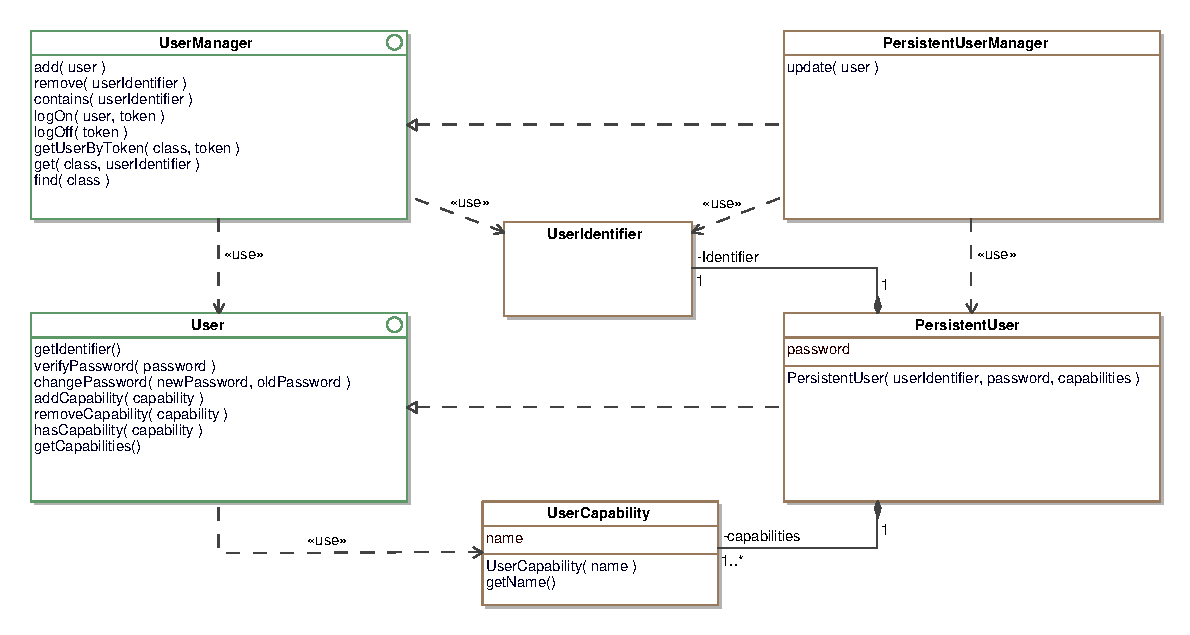
\includegraphics[width=1.0\textwidth]{images/User_Overview.eps}
	\label{user_overview}
	\caption{User - Class Overview}
\end{figure}

Although \code{Shop} (Section \ref{shop}) holds a reference to a \code{UserManager}, \code{PersistentUserManager} does not need to be a singleton instance and is indeed not.
Moreover, a peculiarity of \code{PersistentUserManager} is, that a new instance can be created whenever one is needed.
The reason for this behaviour is, that data is not stored inside the \code{PersistentUserManager} object itself, as it may be done with a collection-based implementation, but \code{PersistenUserManager} is merely a transparent interface to the JPA.\\

\subsection*{UserCapabilities}
Capabilities in conjunction with a \code{HasCapabilityTag} (Section \ref{spring}) can be used to change the appearance of a View, depending on a users status.
For example, a View for a user having an ``administrator'' capability may display different content, for example delete buttons, than for a user not having that capability.
Thus, capabilities allow for flexibility and assist in code reuse, when designing the View.
%Extensibility is achieved by using capabilities in conjunction with the \code{Has, which are aggregated by \code{User}s.

\subsection*{Login}
To reduce code repetition, \salespoint{} contains code to automate user log in.
Using a JSP template, a special login form is generated, which is handled by an interceptor.
\footnote{An interceptor is a Spring concept.}
The interceptor verifies the user password and associates the current session with the user.
The session is required, because multiple users can be logged in at the same time.\\

To modify the content of the View, depending on wether a user is logged in or not, the \code{LoggedInTag} can be used.
